%!TEX root=paper.tex


  \newpage
  \section{Service Utilization and Performance}

  Since it is taylored for Flask applications, to deploy the \tool one simply needs to use one line of code\footnote{We don't count the import statement that enables that line...} to bind the dashboard to their Flask web application\footnote{\ins{ In this paper we present the integration with APIs written in Python and Flask hoping that this will not prevent the reader from seeing the more general idea; all the tools we show here for Flask can be applied to other API technologies (e.g. Django) by simply providing a few back-end adapters in the right places. }}:

  % caption=Configuring the \tool is straightforward,
  \begin{lstlisting}[style=custompython]
  import flask_monitoringdashboard as dashboard

  # LOC #1: associate the main Flask application 
  # object with the dashboard
  dashboard.bind(app) 

  \end{lstlisting}


  During binding, the \tool will search for all endpoints defined in the target application 
    \ins{ 
      and add function wrappers around all the corresponding endpoint functions
    }
% 
  % In order to monitor an endpoint, the \tool creates a function wrapper for the API function that corresponds to the endpoint. This way, the wrapper will be executed whenever that API call is made before the actual function is called. The wrapper contains the code that takes care of monitoring an endpoint. 
% 

   \ins{
    The tool takes advantage of the fact that the monitored API already has a web presence, and makes available one extra endpoint (i.e. \code{/dashboard}), which serves the interactive visualization perspectives presented in the remainder of this paper. 
  }  
 The first perspective presents all the automatically discovered endpoints and lets the user select the ones that should be monitored. 
  \Fref{fig:sep} shows that the last access time of every endpoint is tracked irrespective of whether it is selected by the user to be monitored or not. 


    \begin{figure}[h!]
      \centering
      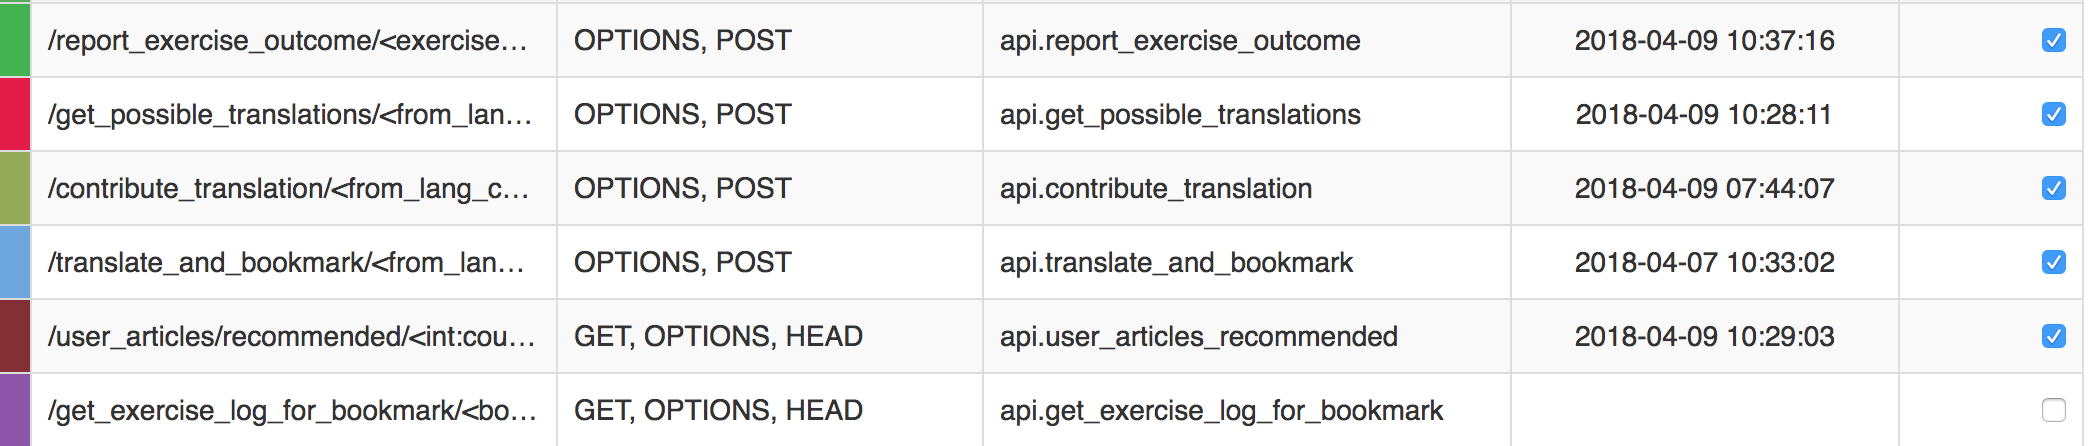
\includegraphics[width=\linewidth]{selecting_endpoints.png}
      \caption{Once connected to an API the Dashboard presents the endpoints that are available for monitoring}
      \label{fig:sep}
    \end{figure}

  \ins{
    We have decided for an opt-in approach to monitoring to avoid any the performance penalties incurred by the dashboard to affect performance sensitive endpoints. We discuss performance issues later. Also, we discuss later one situation in which opt-out might be desirable. 
  }

  \ins{

    One alternative to allowing the user to use annotations would be to let them to annotate the code. However, this pollutes the code, and prevents deploying two versions which would monitor different endpoints. 

  }

\niceseparator

  \ins
  {

      The remainder of this section presents several of the interactive
      visualizations that become available without any further configuration\footnote{We recommend obtaining a color version of this paper for better readability}.

  }
